\section{Evaluation}

This section details how the research proposal will be evaluated, which encompasses the evaluation stage of the DSMR methodology. Piers-Heje et al. differentiates two aspects of the evaluation of an IS artifact: when evaluation takes place and how it is evaluated, meaning the timing and environment of the evaluation. 

Given that the framework described in the research proposal section will be evaluated after it has been constructed and given that the evaluation of the proposed framework will be based on its actual use within a real development scenario, the evaluation will be “ex post” as opposed to “ex ante”, which would evaluate the design of the model before it was constructed and after its design. Since the evaluation will be carried out within an organization in a real-life scenario with real users, and as such in regards to the way the evaluation is conducted, it will be naturalist, in opposition to the artificial environment according to Piers-Heje et al \cite{J.Pries-Heje:2008SD}. The artifact will then be subjected to four types of evaluations, as shown in Figure 6:

\begin{itemize}
    \item \textbf{Demonstration:} The application of the proposed framework in a realistic organizational scenario will provide initial evidence of its usefulness, clarity, and effectiveness in guiding Human--AI collaboration in the context of an organization.
    \item \textbf{Practitioner Interviews:} Interviews with software developers, engineering managers, and AI practitioners will be conducted to collect insights regarding the practicality, feasibility, and perceived value of the framework in real development workflows.
    \item \textbf{Scrum/Agile Expert Interviews:} Agile coaches, Scrum masters, and product development experts will be consulted to evaluate how well the framework aligns with Agile principles, complements existing delivery methodologies, and addresses the emerging challenges of AI-augmented development.
   \item \textbf{Analytical Evaluation using Benchmarks and Success Criteria:} 
    The framework will be evaluated against predefined criteria, including clarity, completeness, alignment with SDLC phases, support for Human-in-the-Loop practices, and governance of AI-enabled activities. Each criterion will be assessed qualitatively using a three-level ordinal scale (low, medium, high), which is commonly used in qualitative DSR evaluations to indicate degree of satisfaction rather than precise performance measurement. Therefore indicating the extent, to which the framework satisfies each criterion, based on evidence gathered from the demonstration and expert feedback, with brief qualitative justifications grounded in observed usage, artifacts, and interview data.
\end{itemize}

\begin{figure}[H]
    \centering
    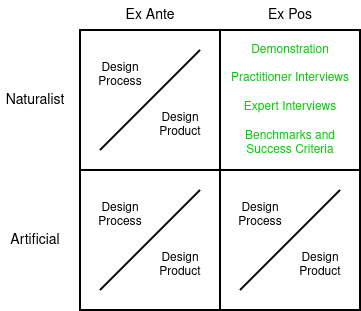
\includegraphics[width=0.33\linewidth]{Images/evaluation.png}
    \caption{Chosen approach for artifact evaluation (adapted from \cite{J.Pries-Heje:2008SD})}
    \label{fig:placeholder}
\end{figure}

The evaluation is expected to provide evidence regarding the practical suitability and perceived value of the proposed framework. It is anticipated that practitioners will highlight strengths such as improved guidance for Human-AI collaboration, clearer role definition, and enhanced structure for integrating AI tools across SDLC activities. Agile experts are expected to comment on how the framework aligns with or extends Agile principles, particularly in environments adopting Vibe Coding or AI-assisted development. However, certain limitations are acknowledged. As the evaluation is conducted within a limited number of organizational settings, broader generalization may be constrained. The scope of real-world application may also be limited by time, availability, or the maturity of AI tools in use. Finally, because the evaluation focuses on early practical adoption, long-term impacts such as organizational change or sustained performance improvements cannot yet be measured.

Despite these limitations, the evaluation is expected to provide a strong foundation for validating the relevance and applicability of the proposed framework and for identifying directions for future refinement and potential large-scale deployment.